% allocation.tex

%%%%%%%%%%%%%%%%%%%%
\begin{frame}{TODS2025 Allocating Isolation Levels to Transactions in a Multiversion Setting}
	\begin{columns}
		\begin{column}{0.5\textwidth}
			\textbf{Problems: }开发人员手动为每类的事务选择隔离级别具有挑战性。选择过于保守,会严重影响吞吐量;选择较低的隔离级别,则需要复杂的并发逻辑来避免异常。

			\textbf{Contributions: }一种在多版本数据库中系统性地分配隔离级别给事务的框架,能够根据事务行为,自动分配最合适的隔离级别,在确保在所需正确性的前提下最大化性能。
		\end{column}
		\begin{column}{0.5\textwidth}
			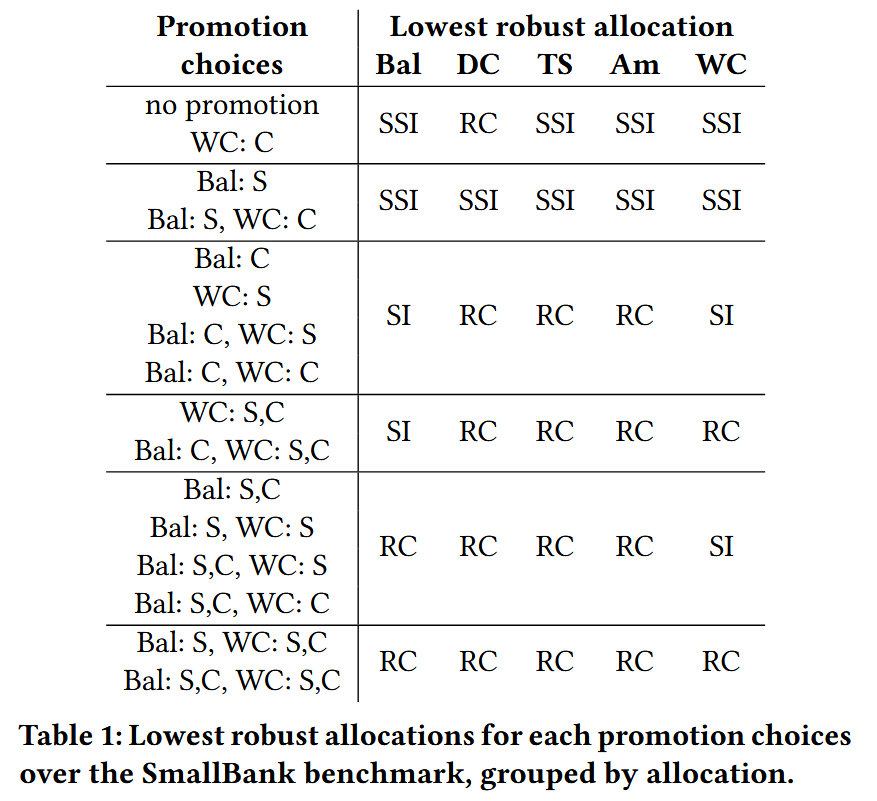
\includegraphics[width=0.98\linewidth]{figs/lowest-robust-allocations}
		\end{column}
	\end{columns}
\end{frame}
%%%%%%%%%%%%%%%%%%%%

%%%%%%%%%%%%%%%%%%%%
\begin{frame}{TODS2025 Allocating Isolation Levels to Transactions in a Multiversion Setting}
	\begin{columns}
		\begin{column}{0.5\textwidth}
			\textbf{Basic Ideas: }分析事务的访问模式(读集和写集),动态识别潜在的冲突依赖环:
			\begin{itemize}
				\item 对只读事务,安全分配 RC 以实现高吞吐量;
				\item 对可能产生依赖环的事务,自动提升隔离级别至 SI 或 SER;
				\item 结合静态分析与运行时监控,在事务执行前/期间动态决策隔离级别。
			\end{itemize}
		\end{column}
		\begin{column}{0.5\textwidth}
			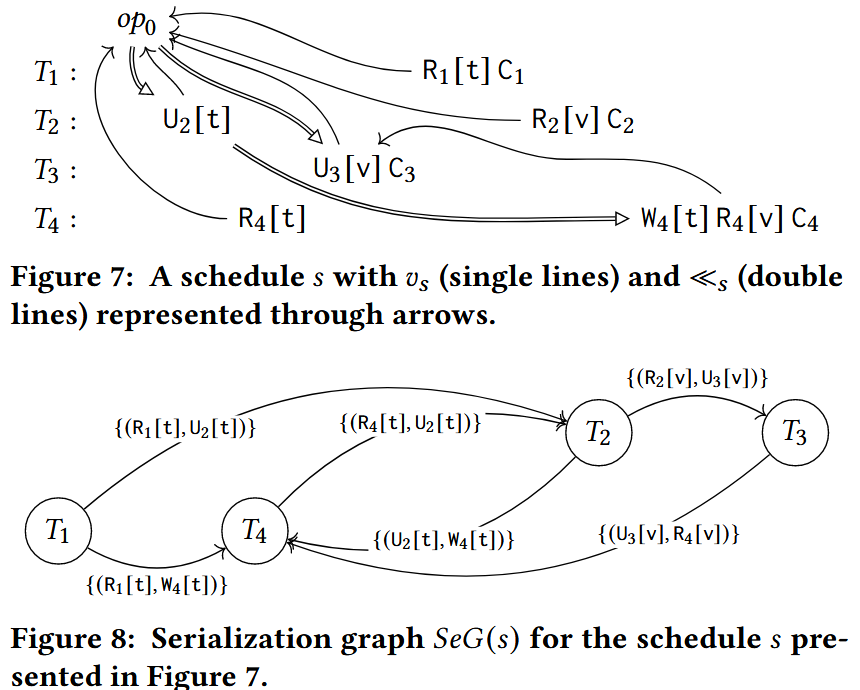
\includegraphics[width=0.98\linewidth]{figs/confliction-detect}
		\end{column}
	\end{columns}
\end{frame}
%%%%%%%%%%%%%%%%%%%%

%%%%%%%%%%%%%%%%%%%%
\begin{frame}{TODS2025 Allocating Isolation Levels to Transactions in a Multiversion Setting}

	\textbf{Limitations: }
	\begin{itemize}
		\item 依赖调度分析,不支持分布式数据库;
		\item 执行前的分析引入额外的开销;
		\item 在高度冲突的工作负载下性能优势减弱。
	\end{itemize}

\end{frame}
%%%%%%%%%%%%%%%%%%%%